\newpage
\subsection{Indflydelse af basrefleksens længde}
I dette afsnit vil der blive set på, hvordan længden af basrefleksen kommer til, at spille en rolle i kabinettets samlede frekvenskarakteristik. For at holde variabel-kontrol, så bliver der i første omgang kun målt på betydningen af længden, når basrefleksen er placeret på forsiden af kabinettet.

Der ønskes målt på to dele af højtalerkabinettet: Membranen og basrefleksrøret. Dette gøres ved, at placere CLIO-mikrofonen helt op ad membranen eller helt inde i basrefleksrøret. De to målinger kommer måske ikke til, at være helt akustiske adskilte, men dette er en fejlkilde man er nødt til at leve med.

I første omgang måles der kun på selve membranen, når basrefleksen sidder på forsiden. Resultaterne af disse målinger bliver opvejet med de målinger som blev fundet når kabinettet var helt lukket (ingen basrefleks). Resultatet af dette ses nedenfor.
\begin{figure}[H]
	\centering
	\vspace{-12pt}
	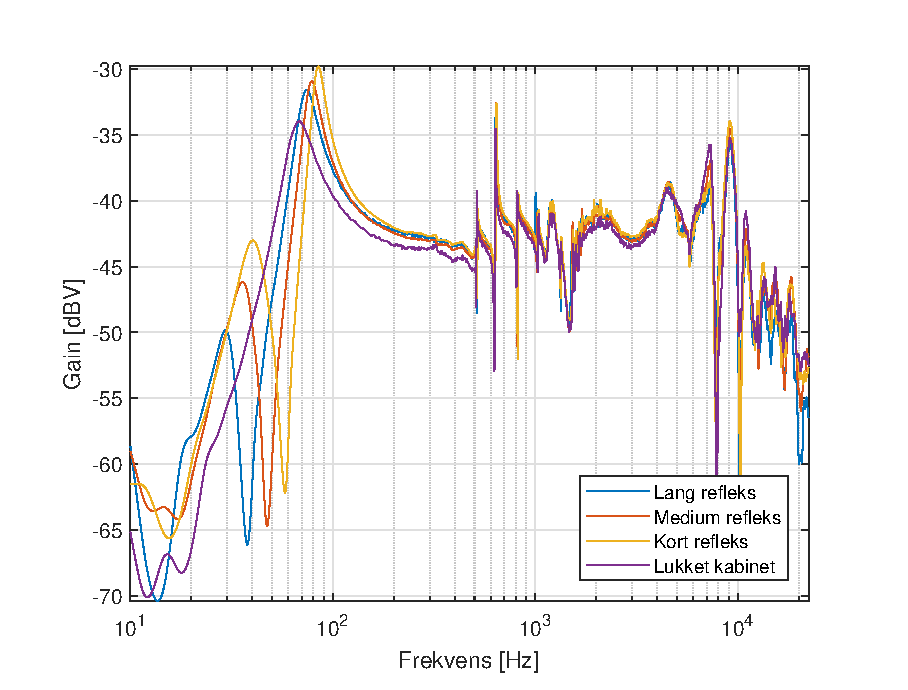
\includegraphics[width=\textwidth]{Billeder/Grafer/BasrefleksLengthMembran}
	\caption{Betydning af basrefleksens længde (målt på membran)}
\end{figure}

Det centrale ved de ovenstående måleresultater er, at der nu forekommer et 'forstærkningsdyk' omkring de lave frekvenser. Samtidig ændres både resonansfrekvensen $f_s$ placering og forstærkningen ved resonansfrekvensen, når der tilføjes en basrefleks eller ændres på længden af basrefleksen.

Det ses på figuren, at jo kortere basrefleksen bliver, jo højere op i både frekvens og forstærkning kommer resonansfrekvensen $f_s$. Samtidig ses det også, at jo længere basrefleksen bliver, jo længere ned i frekvens kommer forstærkningsdykket til at ligge, men at forstærkningen under denne faktisk stiger.

Næste skridt er, at se på selve basrefleksrørets frekvensrespons. Dette respons blev som sagt målt ved, at placere CLIO-mikrofonen inde i selve røret. Af gode grunde, så kan de målte resultater for basrefleksrøret ikke sammenlignes med målte data fra et lukket kabinet.
\begin{figure}[H]
	\centering
	\vspace{-12pt}
	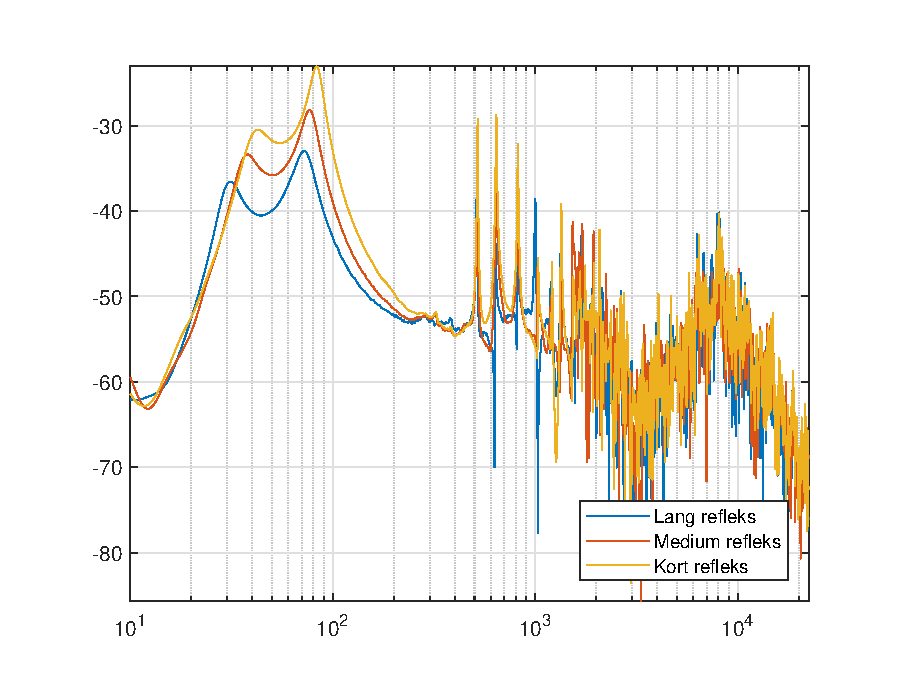
\includegraphics[width=\textwidth]{Billeder/Grafer/BasrefleksLengthTube}
	\caption{Betydning af basrefleksens længde (målt i basrefleks)}
\end{figure}

Den ovenstående figur vil kun blive undersøgt i frekvensområdet fra \SI{10}{\hertz} til \SI{300}{\hertz} idet det er her der ønskes en undersøgelse af basrefleksens indvirkning. Det ses at der optræder to peaks omkring noget der ligner en klassisk båndpaskarakteristik.

Når basrefleksen gøres kortere, så kommer de to peaks til, at give en større forstærkning, men kommer samtidig til, at ligge ved højere frekvenser. Hvis man ønsker en basrefleks der skal give kabinettet et 'løft' ved lave frekvenser, så skal man for dette højtalerkabinet med en lang basrefleks - altså \SI{15}{\centi\meter}.

\newpage
Til sidst blev der set på hvordan en lytter vil opleve lyden fra højtalerkabinettet. Dette blev gjort ved, at placere CLIO-mikrofonen i en afstand på \SI{1}{\meter} fra højtaleren. I dette område burde frekvenskarakteristikken fra membranen og karakteristikken fra basrefleksen ikke længere kunne skelnes, men bør i stedet opveje hinanden.
\begin{figure}[H]
	\centering
	\vspace{-12pt}
	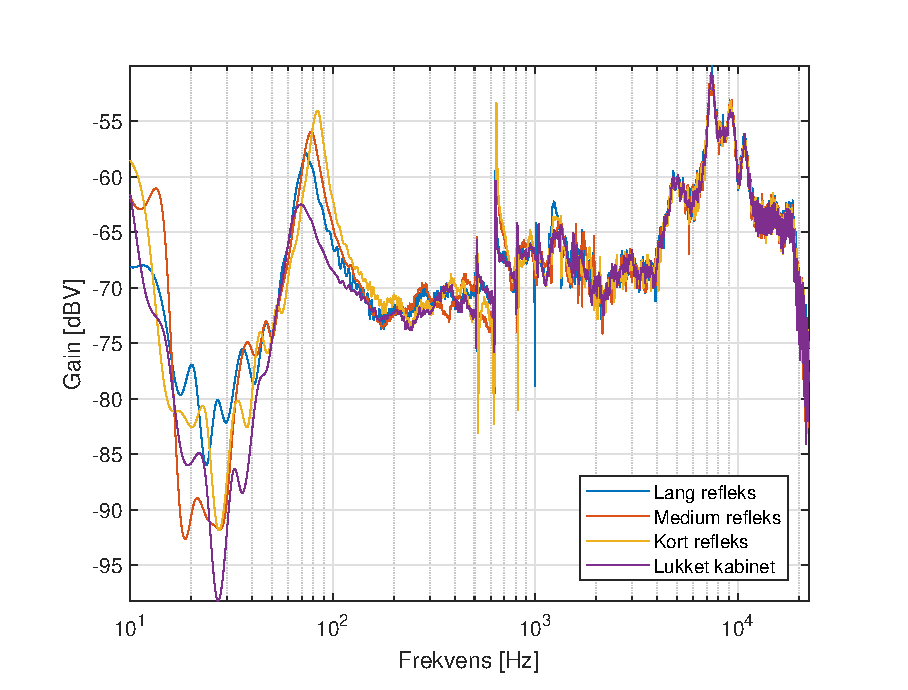
\includegraphics[width=\textwidth]{Billeder/Grafer/BasrefleksLengthFar}
	\caption{Betydning af basrefleksens længde (målt i basrefleks)}
\end{figure}

Det ses, at ved at indsætte et basrefleksrør med længden \SI{15}{\centi\meter}, så stiger forstærkningen ved resonansfrekvensen med omkring \SI{7}{\decibel}. Derudover, så bliver forstærkningen ved de endnu lavere frekvenser (\SI{20}{\hertz} til \SI{40}{\hertz}) også højere med helt op til \SI{15}{\decibel} når der indsættes en lang basrefleks.
\begin{figure}[H]
	\centering
	\includegraphics[width=0.5\textwidth]{Billeder/MaalBasrefleks}
	\caption{Typisk måleopstilling for måling af basrefleksens frekvenskarakteristik}
\end{figure}